

%%%%%%%%%%%%%%%%%%%%%%%%%%%%%%%%%%%%%%%%%%%%%%%%%%%%%%%%%%%%%%%%%%%%%%%%%%%%%%%%%%%%%%%%%%%%%%%%%%%%%%%%%%%%
\section{Evaluation}

We have validated our prototype system, written in C++, on a 64-bit desktop machine with a 3.5 GHz Intel Core I7-3770K processor, 8GB memory, and an Nvidia GeForce GTX 660 GPU video card. \hl{Figure }\ref{fig:MoreRetrievalRes}\hl{ shows retrieval results generated with our method.}

\begin{figure}\centering
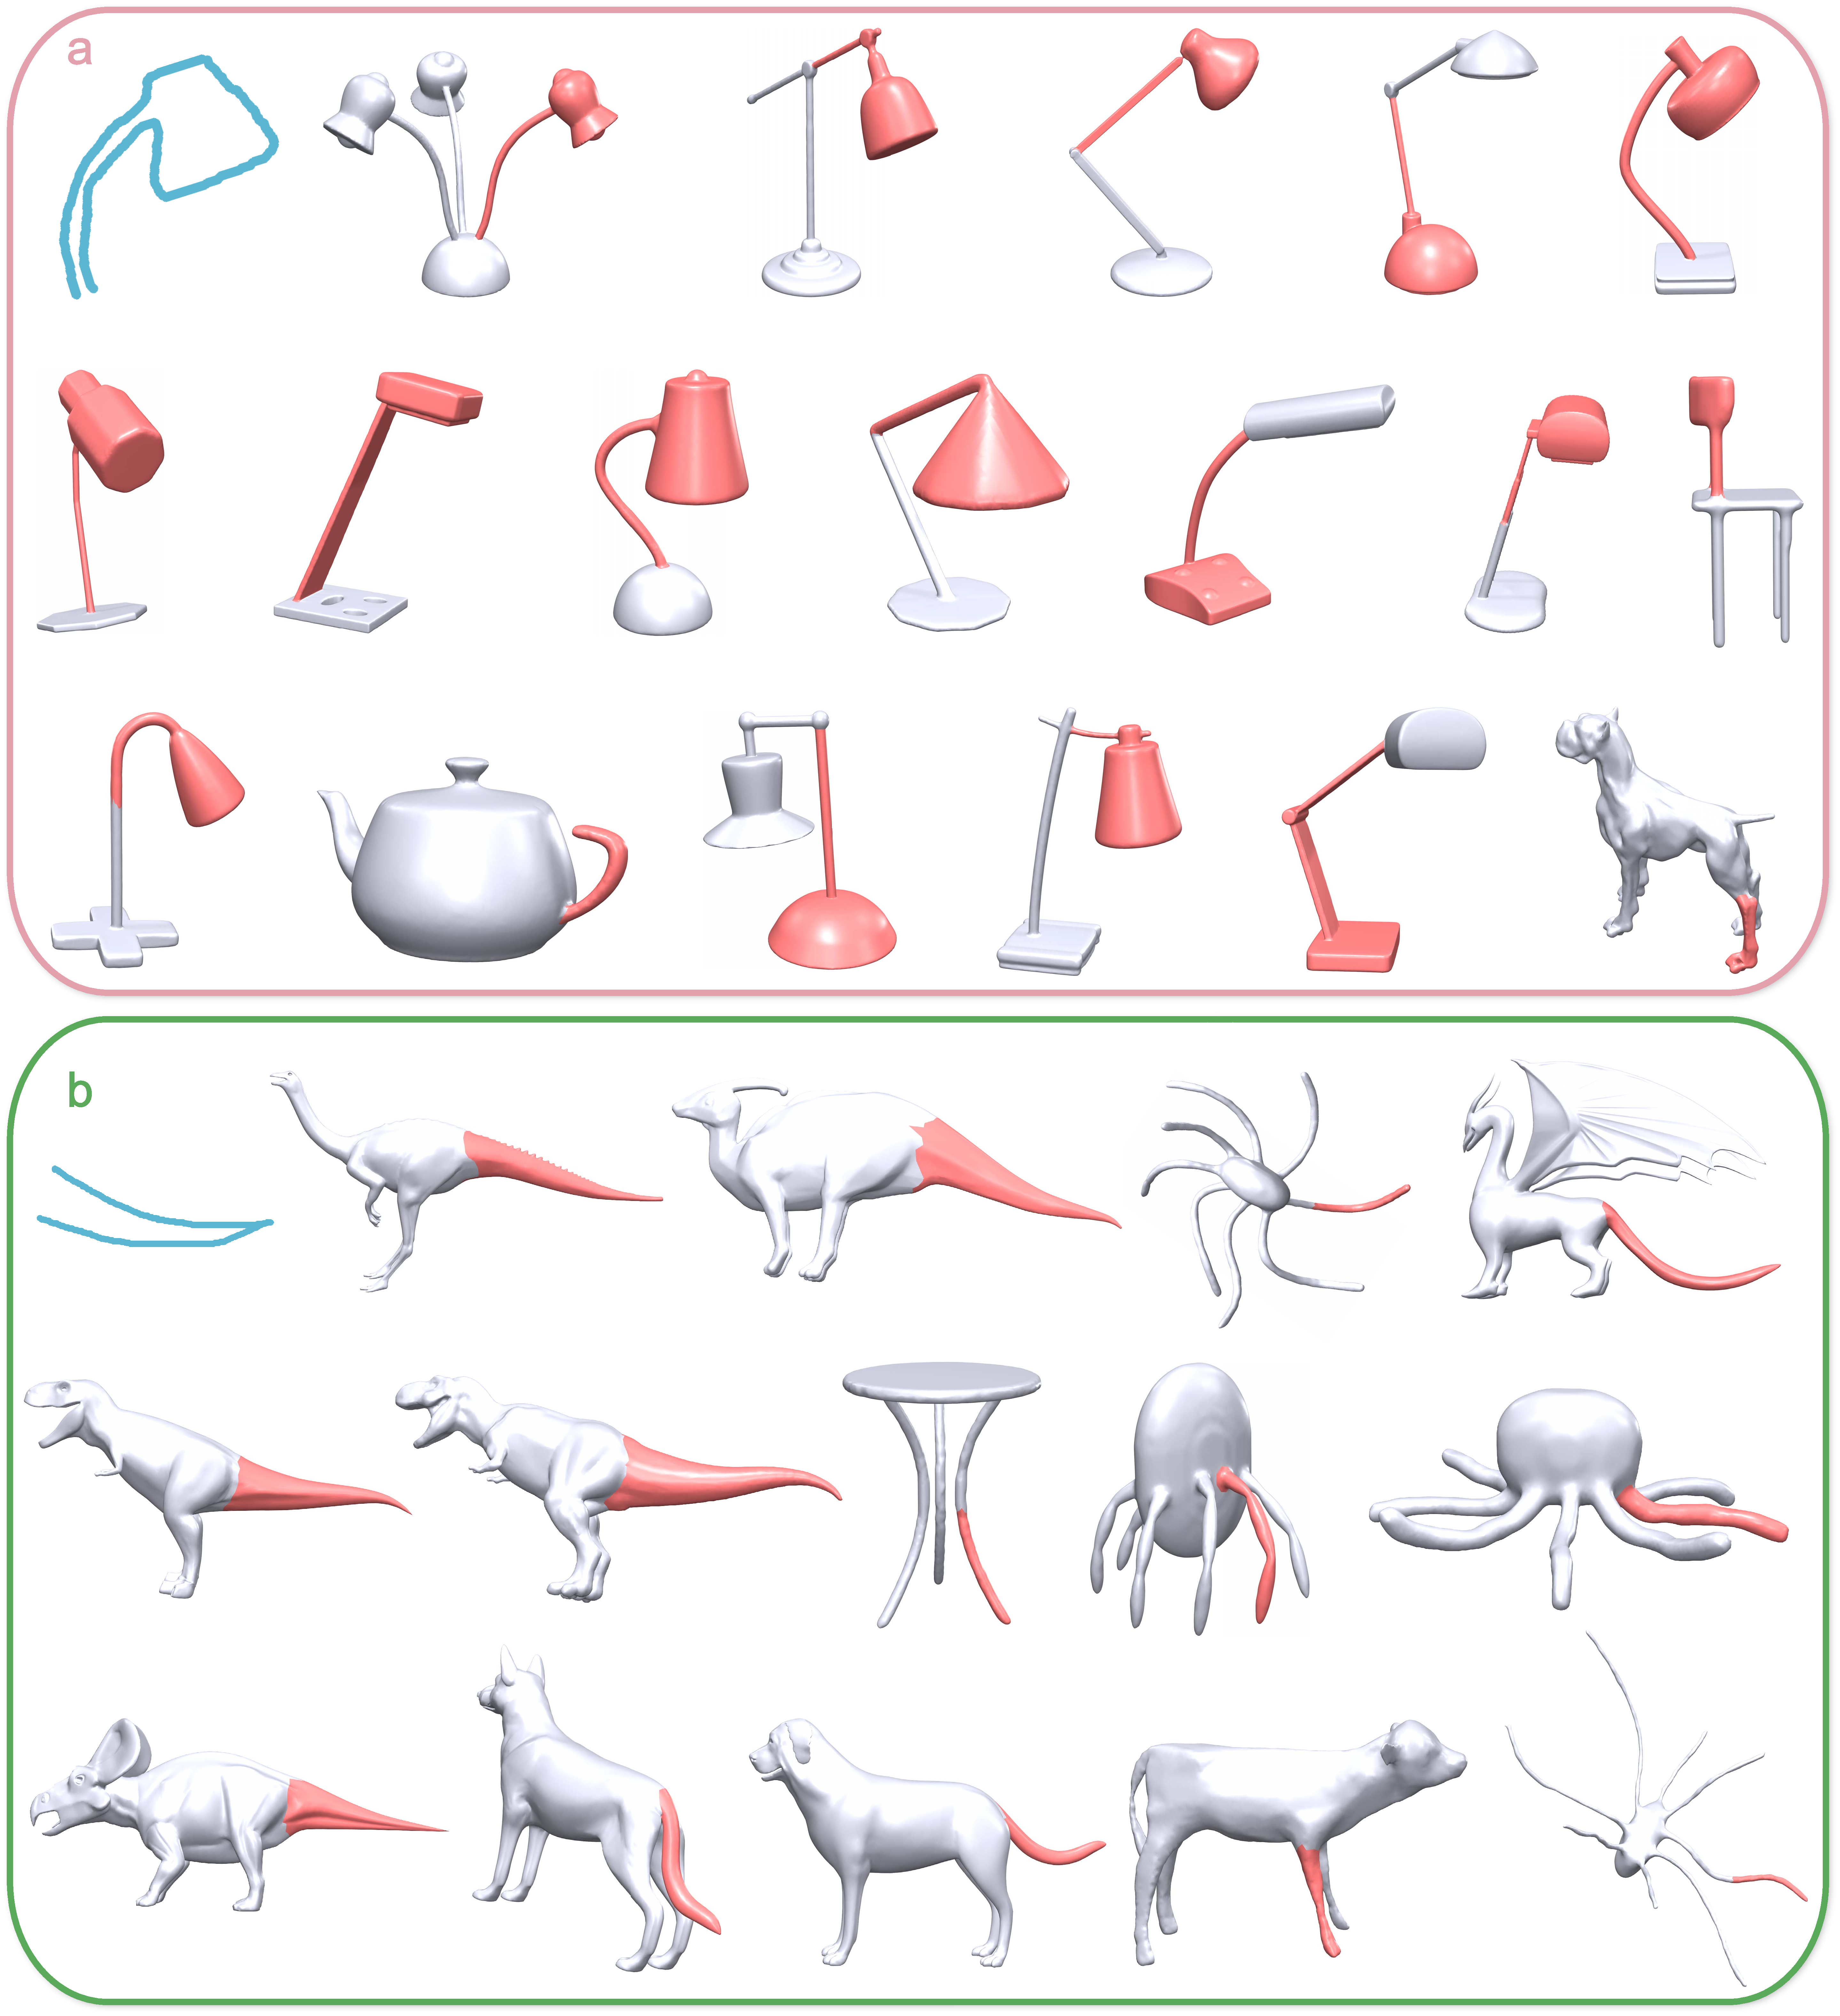
\includegraphics[width=1.05\linewidth]{./Material/MoreRetrievalRes.pdf}
\caption{Retrieval results generated with our method. The retrieved parts are ranked from left to right, form top to bottom.}\label{fig:MoreRetrievalRes}
\end{figure}

There are 513 3D shapes in our database. From these shapes, we extracted 10,773 contours. It took $\sim$3.5 hours to organize these contours into an {\RCKNNG}. The average time to construct the super-face graph of a shape is 20 seconds. Because of the super-face graph representation, our part extraction is real-time. The time for the coarse and fine level extractions for one model is 0.15ms and 10.3ms on average, respectively. Thanks to the two acceleration structures ({\RCKNNG} and SFG) and the coarse-to-fine part extraction strategy, our system can run interactively during the design process. Once a user finishes drawing the sketch, it takes 0.56-0.61 seconds (with GPU and multi-core acceleration) on average for our system to present part suggestions.

\paragraph*{{\RCKNNG} Retrieval Performance.} To evaluate the performance of our {\RCKNNG}, we compare the following methods:
\begin{enumerate}
\setlength{\itemsep}{3pt}
\setlength{\parskip}{0pt}
\setlength{\parsep}{0pt}
\item Traditional (single-layer) $k$NNG constructed by brute force.
\item Wang's randomized $k$NNG approximation~\cite{scalableknnjingwangcvpr2012}.
\item {\RCKNNG} constructed by brute force.
\item {\RCKNNG} with Wang's randomized approximation (\mbox{\textbf{our method}}).
\end{enumerate}
For the two $k$NN graph methods (1 and 2), nodes of the graph are complete shape contours. Node adjacencies and edge weights are identified by global comparison of shape contours. \hl{To compute the contour descriptor of the shape contour, the shape contour is first sampled under 3 different scales. 50, 150, and 250 points along the contour are sampled respectively. The contour descriptor is then calculated for the sampled points.} When searching for partial matches to a query contour, we must extract similar contour sections explicitly, significantly slowing down both methods.

For the two {\RCKNNG} methods (3 and 4), nodes of the graph are contour sections (Section \ref{sec:acc}). In our evaluations, we set $k = 20$  and extract $6$ sections from each shape contour.

The retrieval performance for each method is shown in Table \ref{tab:RCKNNGComp}. It is clear that RC-$k$NNG with Wang's method, as proposed in this paper, has the best performance. For retrieval, it is about 97 times faster than Wang's $k$NNG, with only 3 times the construction time. The $k$NNG approaches, which require explicit partial matching at runtime, are much slower. \hl{ We quantitatively evaluate the quality of the extracted parts by comparing the contour of the extracted parts with the user's sketch in terms of the contour descriptor introduced in Section }\ref{subsec:CtourDesc}\hl{. It is clear that the retrieval quality for the two {\RCKNNG} methods is better than that of the two $k$NN graph methods. We visualize the retrieved parts in Figure }\ref{fig:RCKNNGComp}\hl{. The precision recall curves for the two retrieval methods is shown in Figure }\ref{fig:PreRecCurve}\hl{(a). It is clear that the two {\RCKNNG} methods perform better than the two $k$NNG methods. The reason is that the $k$NNG methods, comparing shape contours in a global manner, may match obviously dissimilar contour sections together.}
%--------------------------
\begin{table}\centering \renewcommand\arraystretch{1.3}
\begin{tabular}{|c|c|c|c|}
\hline \diagbox{Algorithm}{Performance}       & RT     & CT      & ME  \\
\hline BF $k$NNG                              & 4.54s  & 51.7h   & 0.0799   \\
\hline Wang $k$NNG                            & 5.68s  & 1.15h   & 0.081  \\
\hline BF {\RCKNNG}                           & 0.053s & 33.89h  & 0.07  \\
\hline Wang {\RCKNNG}                         & 0.058s & 3.52h   & 0.07  \\
\hline
\end{tabular}
\caption{Retrieval performance for different methods on our test dataset.
RT is the retrieval time for a query contour. CT is the construction time for the data structures. ME is the matching error for the retrieved parts.
BF $K$NNG represents the Brute force $k$NNG method. Wang $k$NNG represents the Wang's $k$NNG approximation method.
BF {\RCKNNG} represents the {\RCKNNG} with the brute force method.
Wang {\RCKNNG} represents the {\RCKNNG} with Wang's method.}\label{tab:RCKNNGComp}
\end{table}
%--------------------------
\begin{figure} \centering
\includegraphics[width=1.0\linewidth]{./Material/RCKNNGComp.pdf}
\caption{Retrieved parts generated with different methods: the brute force $k$NNG method (a), the Wang's randomized $k$NNG approximation method (b),
the {\RCKNNG} with the brute force method (c), and the {\RCKNNG} with Wang's method (d).}
\label{fig:RCKNNGComp}
\end{figure}
%--------------------------
\begin{figure}\centering
\subfigure[Different retrieval methods]{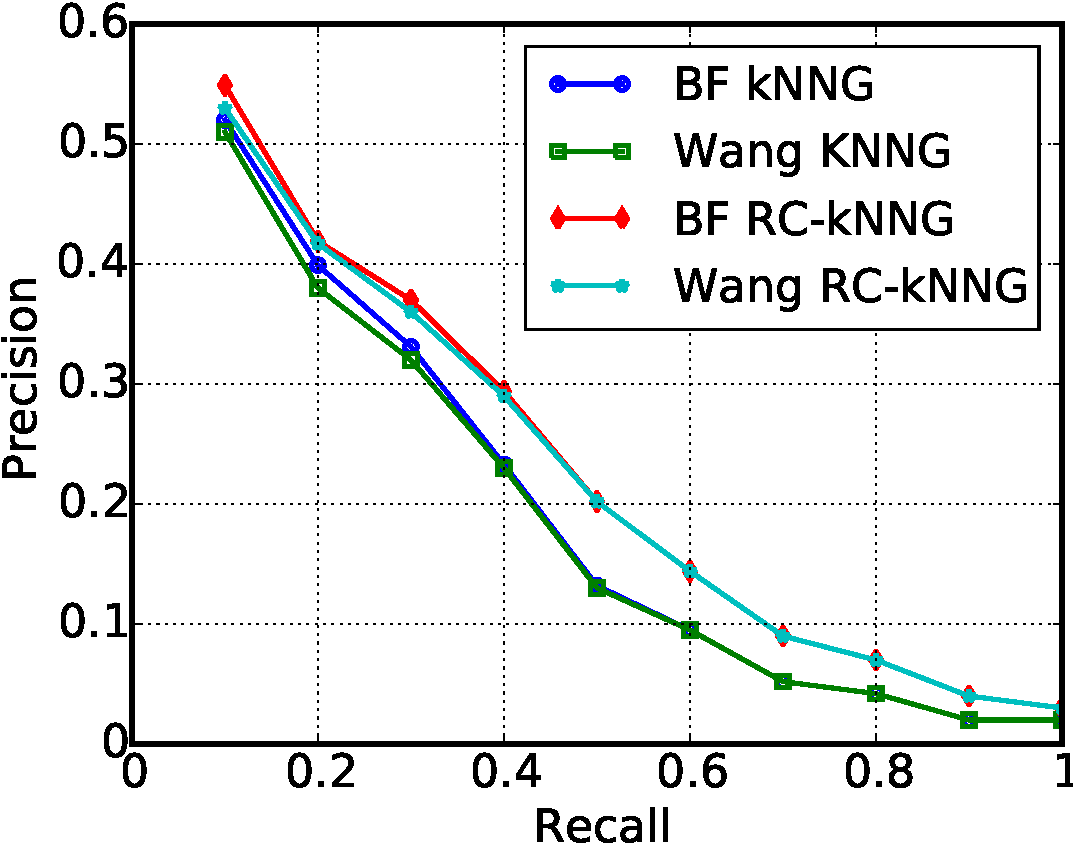
\includegraphics[width=0.49\linewidth]{./Material/PreRecDifAlg.pdf}}
\subfigure[Different camera view settings]{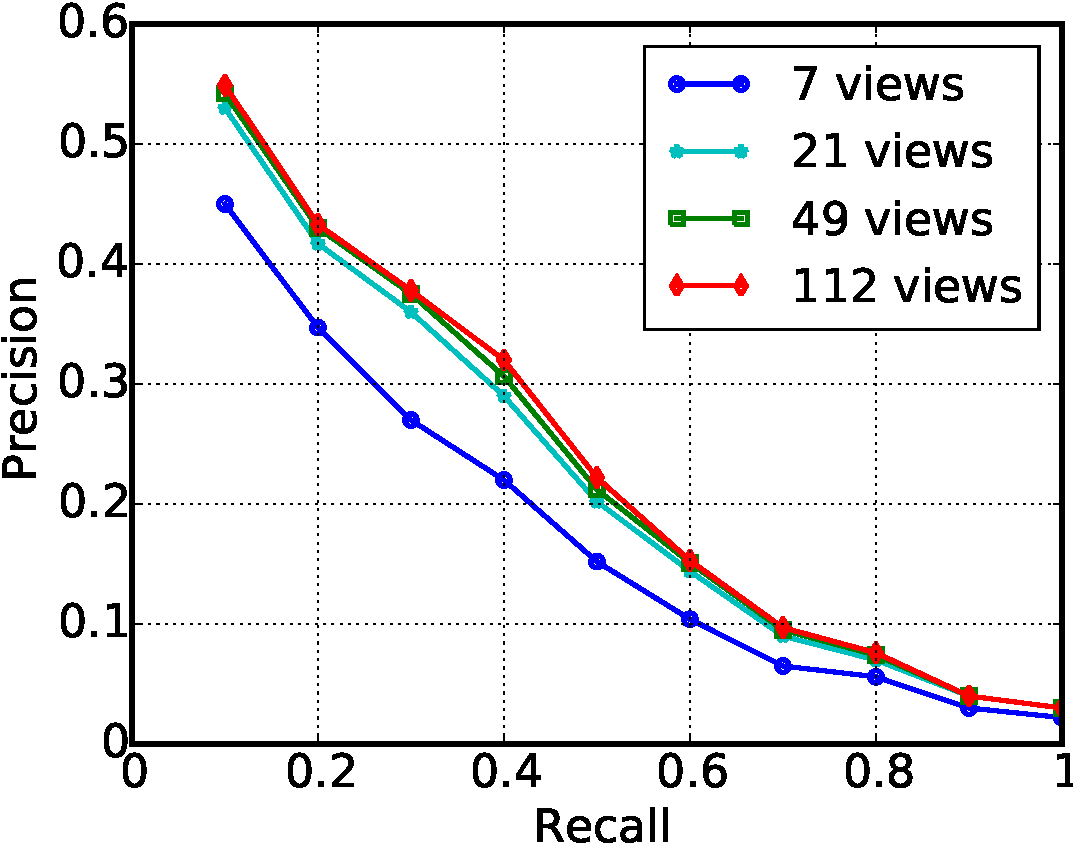
\includegraphics[width=0.49\linewidth]{./Material/PreRecDifViews.pdf}}
\caption{Averaged precision recall curves. (a) shows the precision recall curves generated with different retrieval methods on a set of 35 test sketches.
(b) shows the precision recall curves generated with different camera view settings.
In (a), BF kNNG represents the Brute force $k$NNG method; Wang kNNG represents the Wang's $k$NNG approximation method;
BF RC-kNNG represents represents the {\RCKNNG} with the brute force method;
Wang RC-kNNG represents the {\RCKNNG} with Wang's method.}\label{fig:PreRecCurve}
\end{figure}

\paragraph*{Increasing Super-Face Counts.} In Table \ref{tab:SFCounts}, we show the timing statistics for different super-face counts. The coarse-level part extraction time is strongly dependent on the number of super-faces. However, this is a relatively fast step so this dependence does not significantly hurt overall performance. Overall, despite quadrupling the number of super-faces, part extraction remains interactive, completing in well under 1s.

In Figure \ref{fig:SFCountsPartQuality}, we show the qualitative improvement in part extraction as we increase the number of super-faces. With fewer super-faces, the search space is relatively coarse and the extracted parts need not perfectly match the sketch. As we increase the number of super-faces, the search space becomes more fine-grained. The part contours match the sketch better and better, and the part boundaries are less constrained to follow suboptimal cuts. Table \ref{tab:MatchError} shows the matching error statistics for different super-face counts. Note that the error decreases substantially as the shape representation becomes more fine-grained.

%--------------------------
\begin{table}\centering \renewcommand\arraystretch{1.3}
\begin{tabular}{|c|c|c|c|}
\hline \diagbox{Step}{SF Count} & 50    & 100    & 200    \\
\hline Construction of SFG      & 20s    & 14.01s  & 19.07s  \\
\hline Coarse extraction (per shape)  & 0.15ms  & 0.77ms   & 3.91ms   \\
\hline Full part extraction    & 560ms  & 577ms  & 605ms  \\
\hline
\end{tabular}
\caption{Timing statistics with different super-face counts. Full part extraction measures the time from launch of a query to generation of a final part.}\label{tab:SFCounts}
\end{table}
%--------------------------

%--------------------------
\begin{table}\centering \renewcommand\arraystretch{1.3}
\begin{tabular}{|c|c|c|c|}
\hline \diagbox{}{SF Count} & 50    & 100    & 200    \\
\hline Matching error      & 0.45     & 0.29   & 0.07   \\
\hline
\end{tabular}
\caption{Matching error statistics with different super-face counts, averaged over a set of 20 test sketches.}\label{tab:MatchError}
\end{table}
%--------------------------

\begin{figure}\centering
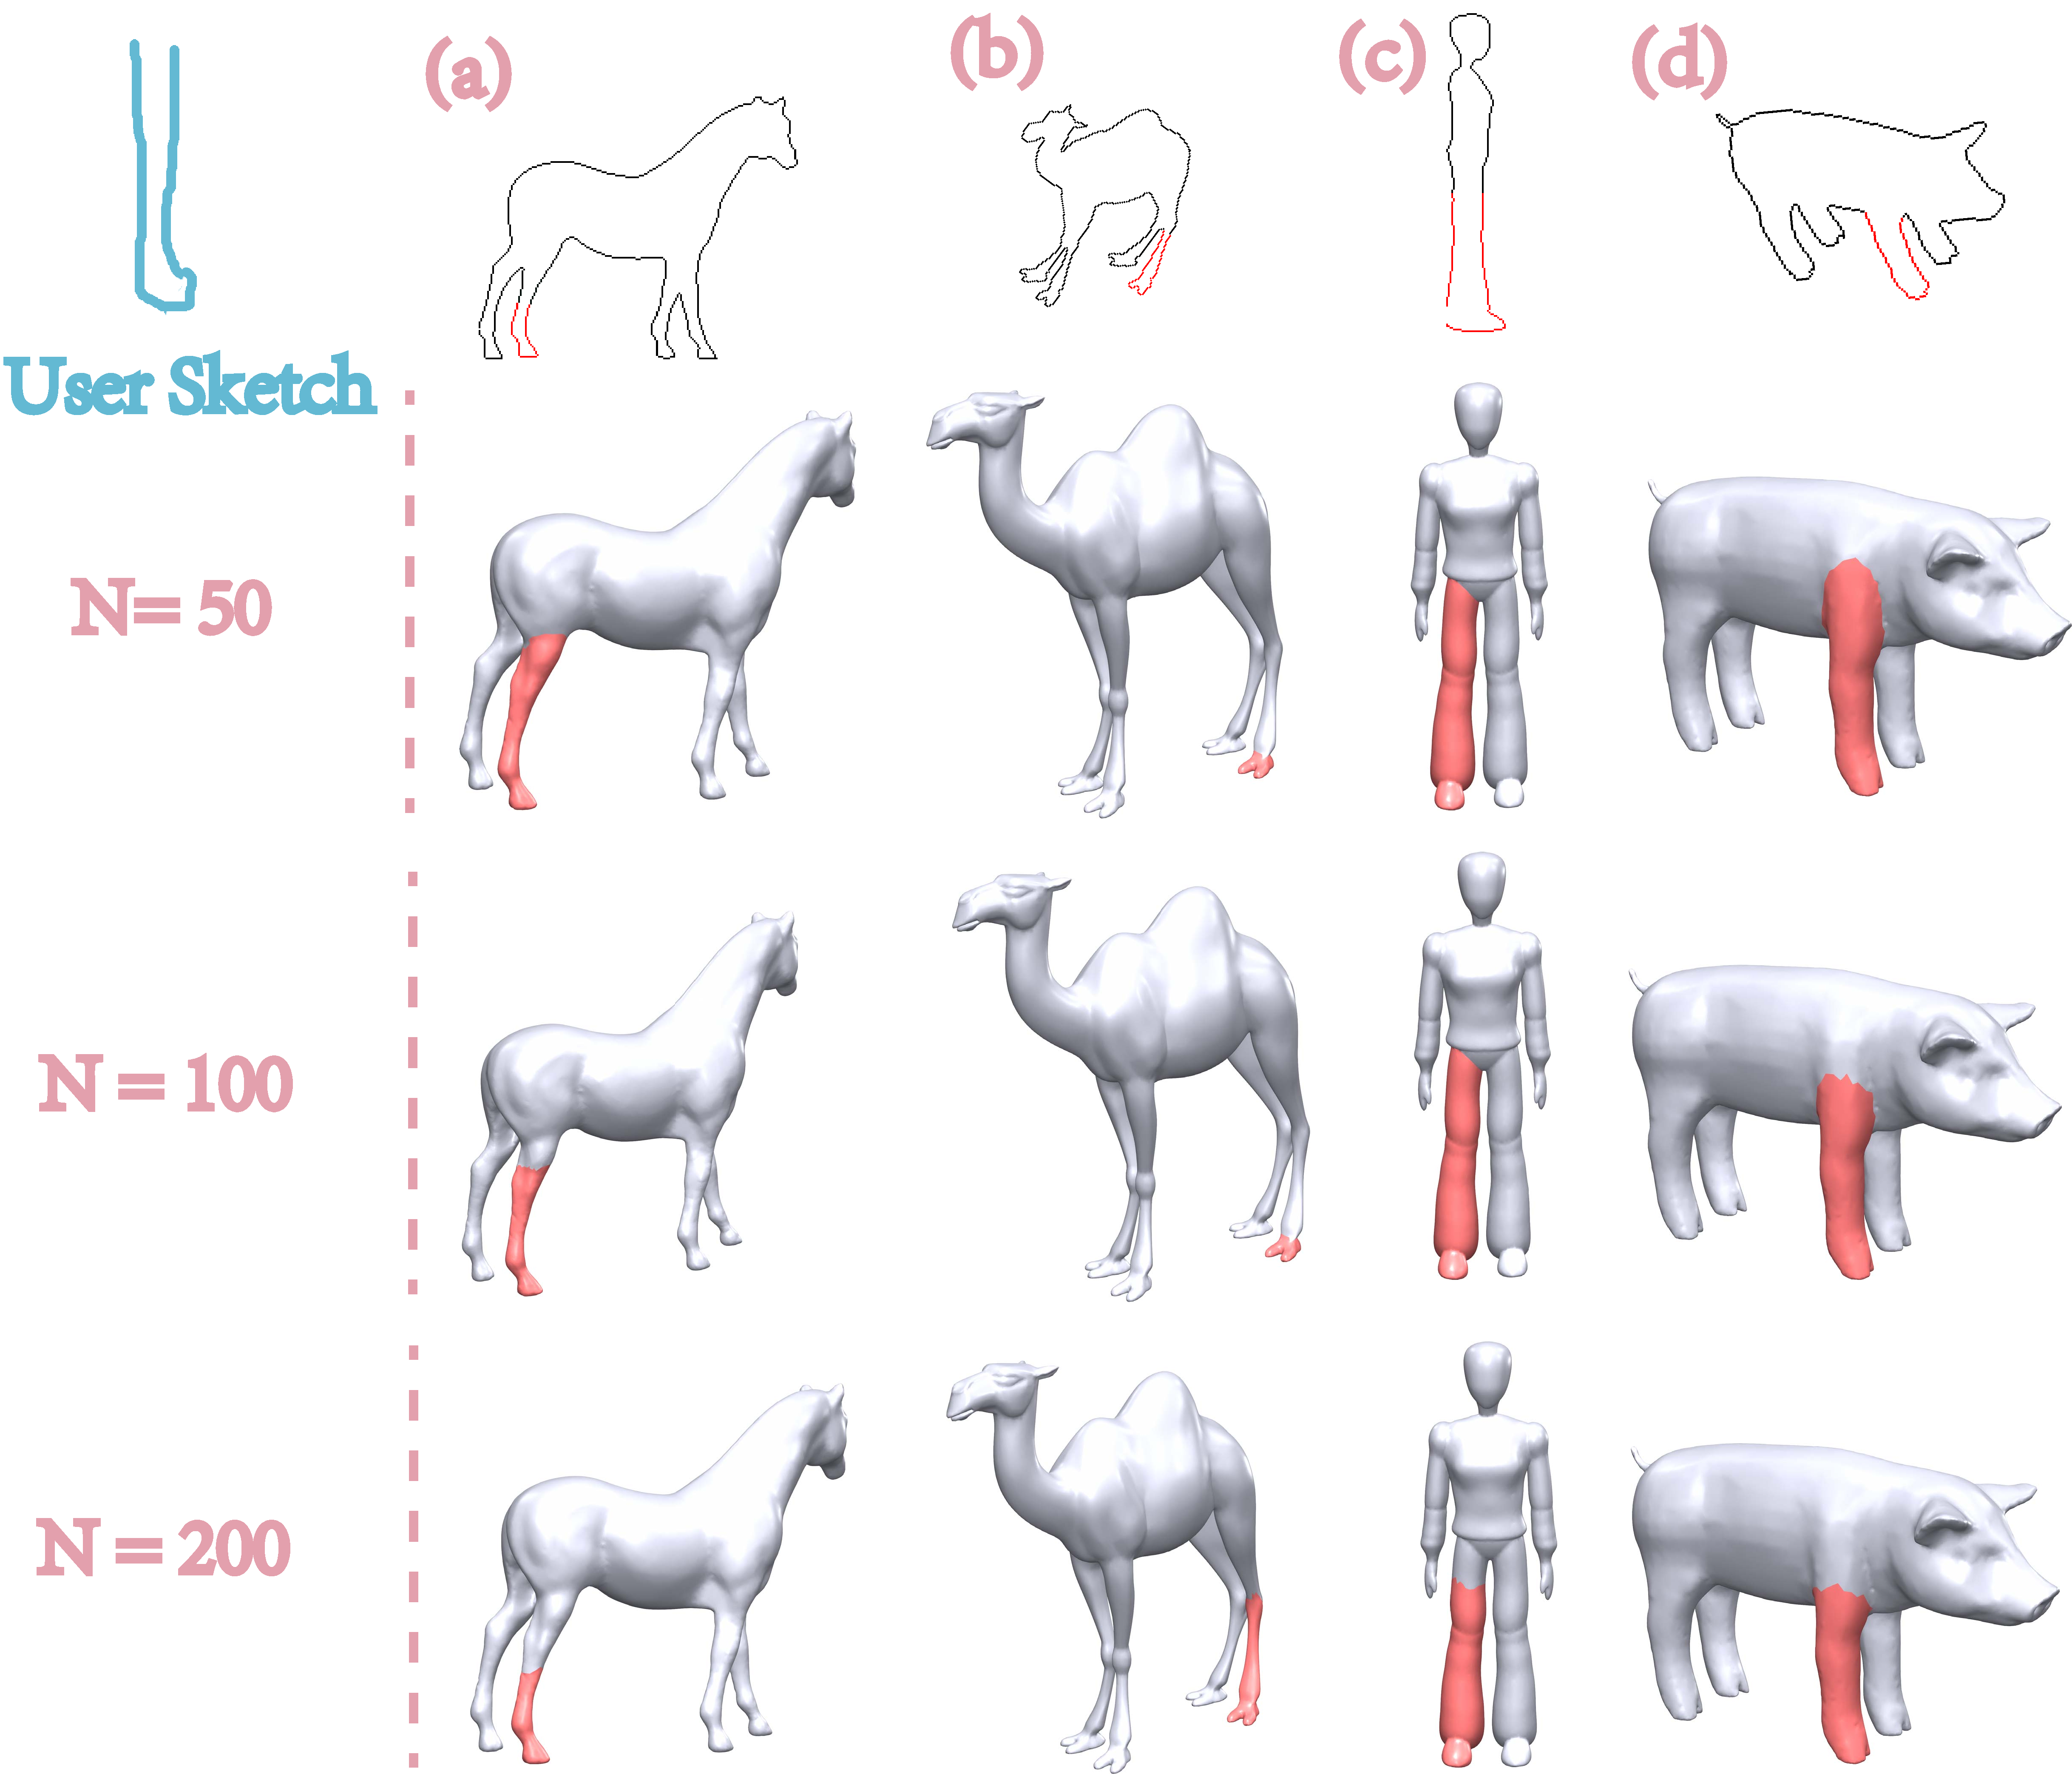
\includegraphics[width=1.0\linewidth]{./Material/SFGNVary.pdf}
\caption{Improvement in part quality with increasing super-face count (N). With more super-faces, the extracted part fits the user's sketch better and better.}
\label{fig:SFCountsPartQuality}
\end{figure}

\paragraph*{Comparison to pre-segmentation approach.}\hl{ We compare our method to the pre-segmentation approach (the method depending on the pre-segmented database). The pre-segmentation method is performed as follows: 1). Each database model is pre-segmented into regular (typical semantic) parts. For example, a human model is decomposed into four parts: head, torso, arms, and legs. 2). We extract boundary contours for each part under different camera views. 3). We construct the $k$NN graph for the part contours. The node in the $k$NN graph represents the whole-part contour. The edge is established by global matching between part contours. 3). In the runtime stage, given the user's sketch, candidate parts are retrieved through a similar procedure as our method with the only difference that contour matching is performed in a global manner. The matching error for the pre-segmentation method is 0.624 averaged over the set of sketches used to generate Table } \ref{tab:MatchError}\hl{. We could clearly find that our method generates better results than the pre-segmentation method. We visualize the retrieval results generated with our method and the pre-segmentation method in Figure }\ref{fig:Comp2PreSeg}\hl{. The reason why our method is better is that our method extracts parts on-the-fly according to the user sketch, while the pre-segmentation method retrieves predefined parts similar to the user's sketch.}
%--------------------------
\begin{figure}\centering
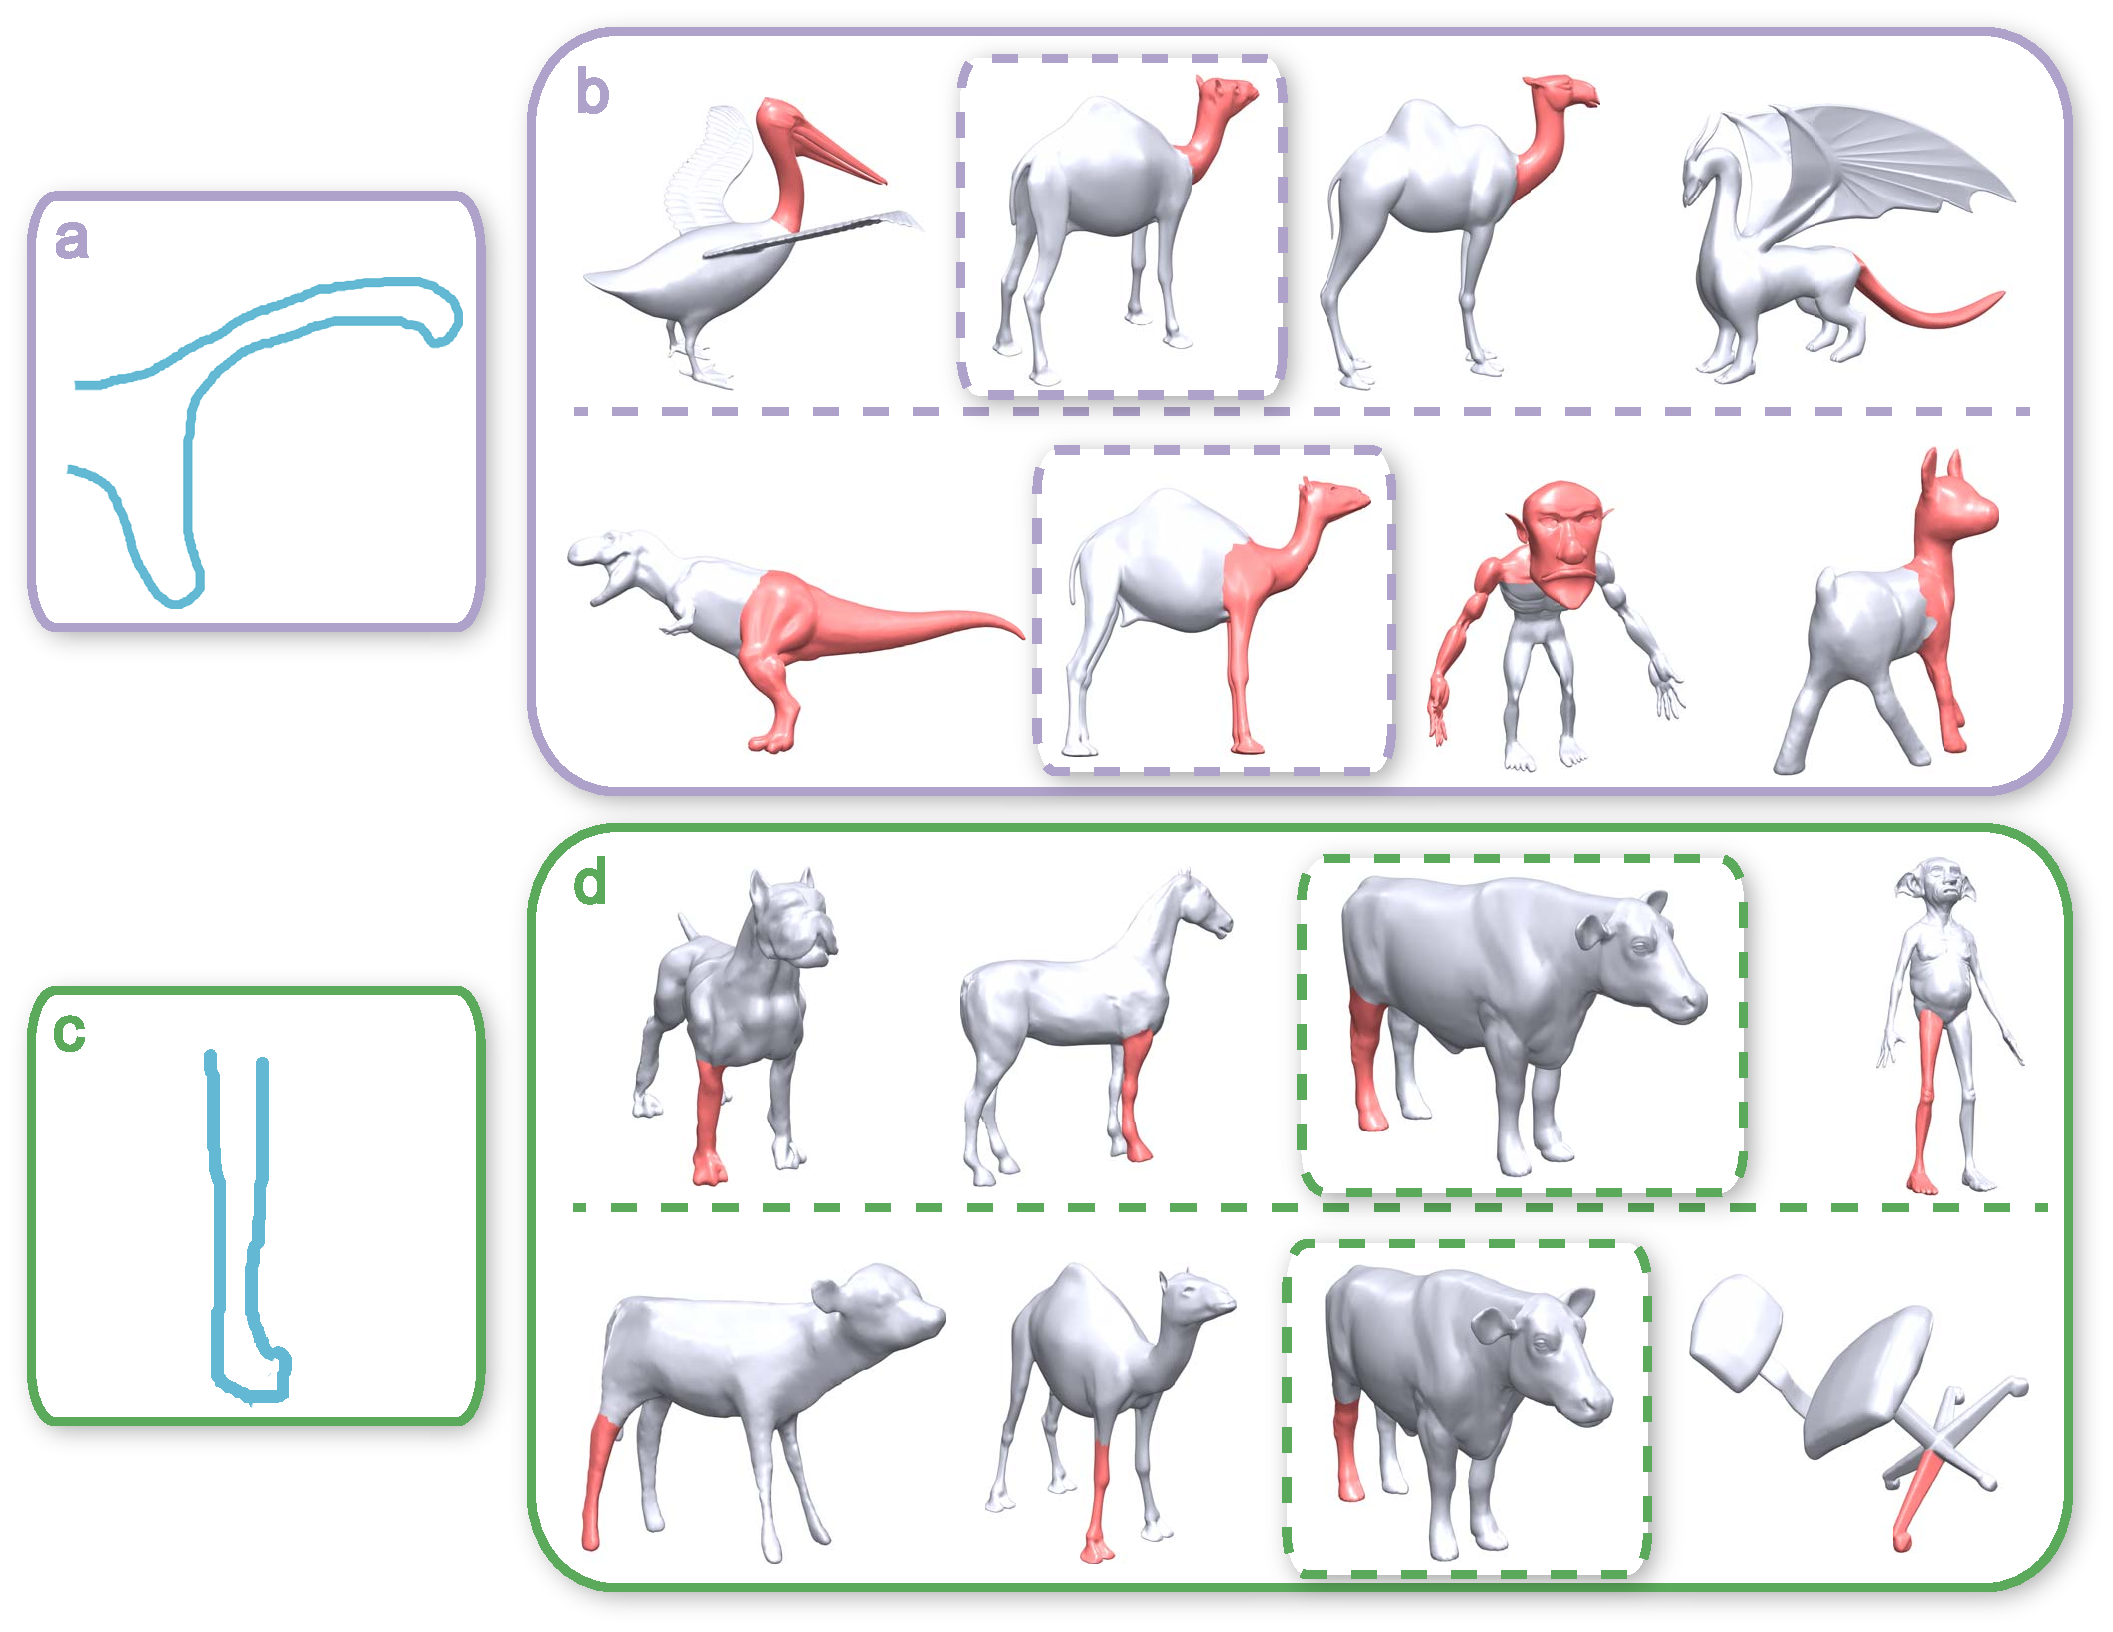
\includegraphics[width=1.0\linewidth]{./Material/Comp2PreSeg.pdf}
\caption{Retrieval results generate with our method and the pre-segmentation method. Given the user's sketch, we show the retrieval results generated with the two methods. In (b) and (d), results generated with the pre-segmentation method are on the upper row; results generated with our method are on the lower row. The pre-segmentation method retrieves the predefined parts (the head of the camel model in (b) and the leg of the cow model in (d)), which is similar to the user's sketch. While our method extracts parts (the ``head+leg'' part of the camel model in (b) and the lower leg of the cow model in (d)) on-the-fly according to the user's sketch.}\label{fig:Comp2PreSeg}
\end{figure}

\paragraph*{Camera view settings.} \hl{We evaluate the influence of the different camera view settings under which we extract contours for the database models. Figure }\ref{fig:PreRecCurve}\hl{(b) shows the precision recall curve generated with different camera view settings. The 7 views include 3 canonical side views and 4 corner views. The 21 views include 3 canonical side views, 4 corner views, and 14 uniformly sampled views}~\cite{FanWang2013}\hl{. The 49 views include 3 canonical side views, 4 corner views, and 42 uniformly sampled views. The 112 views include 3 canonical side views, 4 corner views, and 105 uniformly sampled views. To balance between efficiency and effectiveness, we use 21 views for all the experiments and applications.}s